\documentclass{article}
\usepackage{graphicx}
\usepackage{fullpage}

\title{Approaches to Scamming PageRank}
\author{Manu Goyal, Don-Wook Shin, Luvsanbyamba Buyankhuu}
\date{\today}

\begin{document}

\maketitle

\section*{Introduction}

The PageRank algorithm we studied in class is an effective way to sort pages by
their relative importance. Unfortunately, there are numerous ways malicious
users can modify the network in order to artificially increase the PageRank
score of desired pages. We explore different exploitations of PageRank in the
context of the Simple English Wikipedia network.

\section*{Methods}

We chose to use the Simple English Wikipedia network of pages, because it was a
somewhat large, real-world dataset, but wasn't so large that experimenting with
the data would become too cumbersome. The first thing we did was to calculate
PageRank on the entire wikipedia network, using the standard PageRank algorithm
(which we found on Wikipedia). After looking over the results we got, we devised
two ways to scam the PageRank algorithm, to boost the rank of a specific page.

\subsection*{Method 1: Create Links From Important Pages}

This method is fairly straightforward. Since the rank of a page improves when
other pages with a high rank link to it, somebody could easily improve the rank
of a given Wikipedia page by linking other important pages to it.

To see exactly how much this would improve the score, let $\pi_l$ be the rank of
a low-ranked page, and $\pi_h$ be the rank of a high-ranked page that we will
add a link to. Initially, after PageRank has converged $\pi_l$ will satisfy the
equation $\pi_l = (1 - d) + d(\sum_{i=0}^n \frac{\pi_i}{L(i)})$, where $d$ is a
damping factor for successive iterations of PageRank, $\pi_0 \ldots \pi_n$ are
the ranks of pages that link to $l$, and $L(i)$ is the number of outbound links
for page $i$. Then adding a link from page $h$ would make the rank of $l$
approximately
$(1 - d) + d(\sum_{i=0}^n \frac{\pi_i}{L(i)} + frac{\pi_h}{L(h)+1})$, which is a
difference of $d \frac{\pi_h}{L(h)+1}$. It is important to note that this is not
an exact difference, because adding a link in the network will change the
pageranks of everything else, so the effect on $l$ will be slightly different.
However, as we'll see, this estimate is usually very close to the actual change
in pagerank.

We built a tool, that, given a wikipedia page and a target page rank to improve
to, will suggest a series of pages to add links to, in order to boost the
pagerank to the desired amount. The effectiveness of this tool is explored in
the next section.

\subsection*{Method 2: Create New Pages with High Page Ranks}

While the previous approach could work in the context of Wikipedia, where most
users have access to most of the pages, in many scenarios, malicious users may
have edit access to a very small set of pages. Therefore, we developed a second
way by which to increase the pagerank of a desired page. The idea is to create a
number of pages, each which link to each other in a sequence. Then, we link one
existing page in the network to the first created page in the sequence, and we
will have a sequence of pages with approximately the page rank of the existing
page. Finally, we link all of these created pages to the one we want to improve
the rank of.

To see why this would work, note that with the standard pagerank algorithm, the
amount of pagerank that a page transfers over to something that it links to is
approximately equal to its pagerank divided by the number of links it has. So if
we have an existing page with rank $\pi_e$ and number of outbound links $L(e)$,
then our first created page, with only one incoming link, will have a pagerank
close to $\frac{\pi_e}{L(e)}$. Then if this created page links to exactly one
more created page and the page we want to boost, the second created page will
have a pagerank of $\frac{\pi_e}{2*L(e)}$. We can continue to do this to create
an arbitrary number of pages with a gradually decreasing pagerank. Then if all
of these created pages links to our target page, we can increase its rank by a
significant amount.

\section*{Evaluation}

\subsection*{Method 1}

The pageranks we obtained ranged from 1 to about 38,000. We ran our tool on
pages with ranks 10, 100, 1000, and 10000, and tried to boost
them each to 1000, 10000, and 100000. We first examine the number of edits necessary for each boost. \\

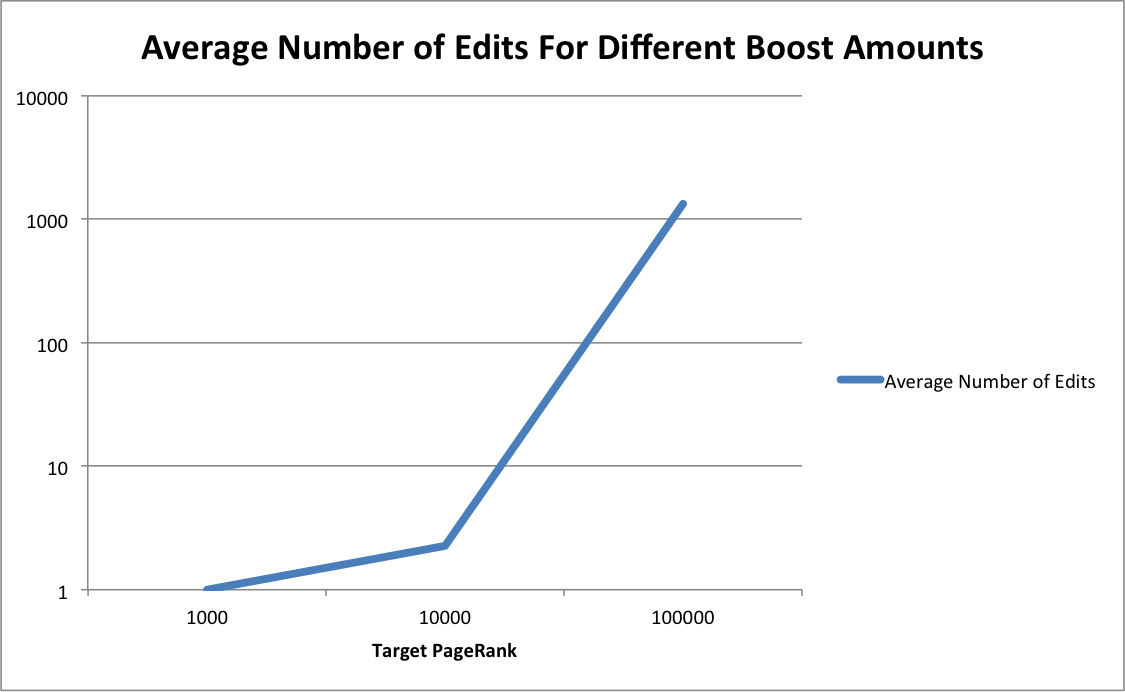
\includegraphics[width=8cm]{EditsPerBoost}

Since there were a number of Wikipedia pages with large existing pageranks, it
didn't take a lot of edits to boost pageranks up to 1000 or 10000, only 1 or 2
edits on average. However, when we wanted to boost up to a rank of 100000, we
needed to edit over 1000 pages on average, primarily because there were only a
few pages that could boost our rank by over 5000, so we needed a lot of less
significant pages to get up to 100000. \\

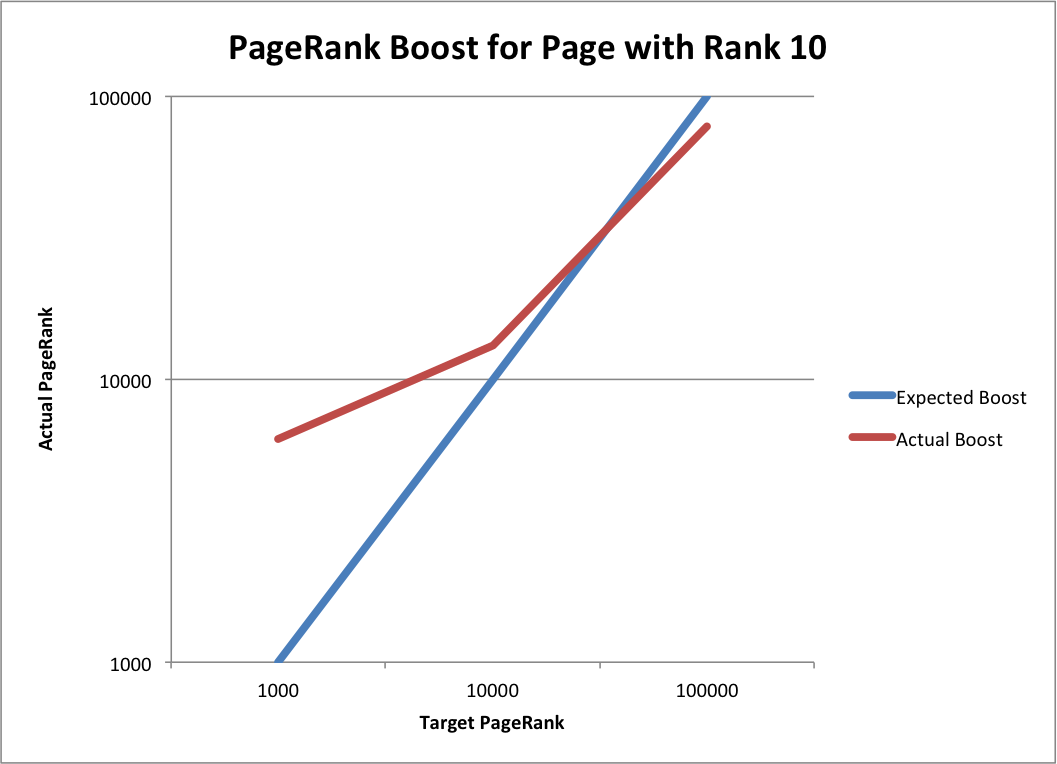
\includegraphics[width=8cm]{PageRank10Boost} 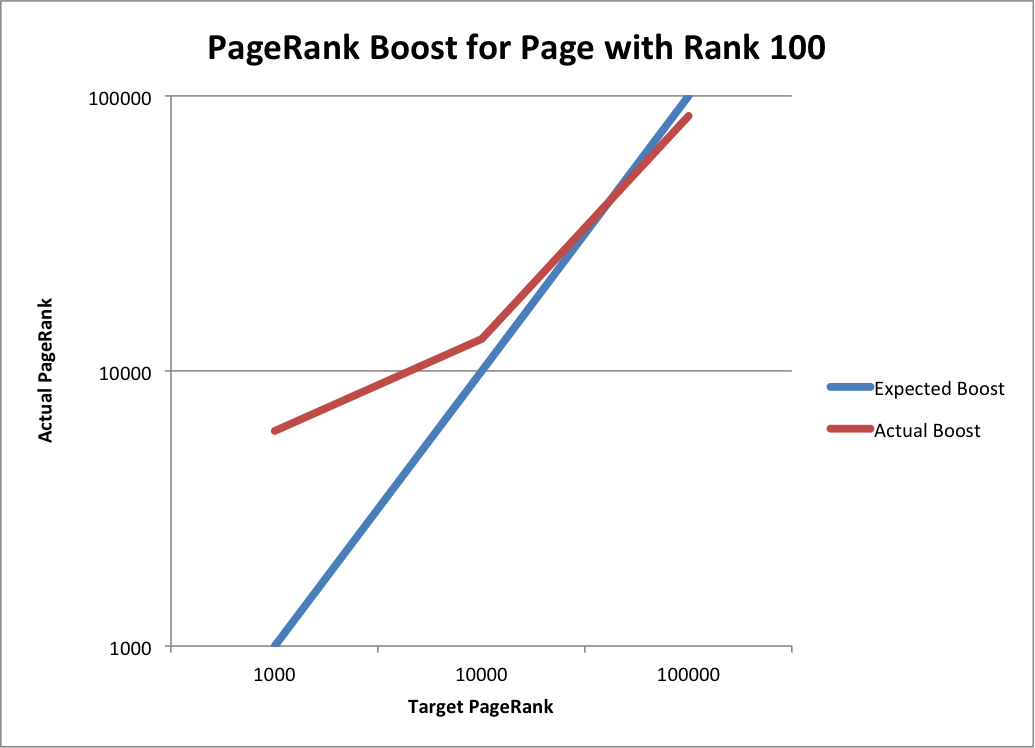
\includegraphics[width=8cm]{PageRank100Boost} \\

Above, we compare the expected and actual boost we got from implementing our
edits, if we started with page ranks 10 and 100 (the graphs for 1000 and 10000
are in the folder, but not in the report for brevity). In both scenarios, our
actual boost exceeded the expected boost when we wanted to increase to 1000 or
10000 (some very large boosts are due to the fact that the algorithm starts by
picking the page that would give the largest boost, rather than the one that
would give a boost closest to what is desired), but when we wanted to increase
to 100000, we fell short slightly. Again, due to the lack of pages that could
lend very large scores to our target pages, we weren't able to reach up to
100000, but the algorithm gets very close.

\section*{Discussion}

Our automated tool for method 1 ended up performing very close to what was
expected. Even though it uses rough calculations to estimate how much linking
pages will affect the pagerank, they tend to be fairly close to the expected
boost, which, in some ways, demonstrates the volatility of the pagerank
algorithm. By adding a very small number of links, we can change the page rank
of specific pages by enormous amounts. The major drawback to this method is that
it is hard to implement in a context outside of wikipedia, where editing large
numbers of important pages is not very feasible.

\end{document}
